\documentclass[a4paper, 12pt]{article}
\usepackage{titling}
\usepackage{array}
\usepackage{booktabs}
\usepackage{enumitem}
\usepackage{graphicx}
\usepackage{hyperref}
\usepackage{amssymb}
%\usepackage{mathtools}
\usepackage{listings}
\usepackage{amsmath}
\usepackage{color} %red, green, blue, yellow, cyan, magenta, black, white
\setlength{\heavyrulewidth}{1.5pt}
\setlength{\abovetopsep}{4pt}
\setlength{\parindent}{0pt}
\graphicspath{{.}}
\usepackage{float}
\usepackage[margin=1in]{geometry}
\definecolor{mygreen}{RGB}{28,172,0} % color values Red, Green, Blue
\definecolor{mylilas}{RGB}{170,55,241}
% Must be after geometry
\usepackage{fancyhdr}
\pagestyle{fancy}
\fancyhf{}
\rhead{NN Homework 9}
\lhead{P.Lukin, E. Ovchinnikova}
\cfoot{\thepage}

\setlength{\droptitle}{-5em}

\title{Neural Networks  \\
				- Homework 9 -}
\author{Petr Lukin, Evgeniya Ovchinnikova}
\date{Lecture date: 21 November 2016}

\begin{document}

%-------------------------------------------------------------------------------
\lstset{language=Matlab,%
    %basicstyle=\color{red},
    breaklines=true,%
    morekeywords={matlab2tikz},
    keywordstyle=\color{blue},%
    morekeywords=[2]{1}, keywordstyle=[2]{\color{black}},
    identifierstyle=\color{black},%
    stringstyle=\color{mylilas},
    commentstyle=\color{mygreen},%
    showstringspaces=false,%without this there will be a symbol in the places where there is a space
    numbers=left,%
    numberstyle={\tiny \color{black}},% size of the numbers
    numbersep=9pt, % this defines how far the numbers are from the text
    emph=[1]{break},emphstyle=[1]\color{red}, %some words to emphasise
    emph=[2]{end,function}, emphstyle=[1]\color{blue},
}

%-------------------------------------------------------------------------------

\maketitle

\section{Mind map}
\begin{figure}[h]
  \centering
  \caption{Mind map. Chapter 6 from Haykin's book. A zoomed version is attached as SVM.png}
  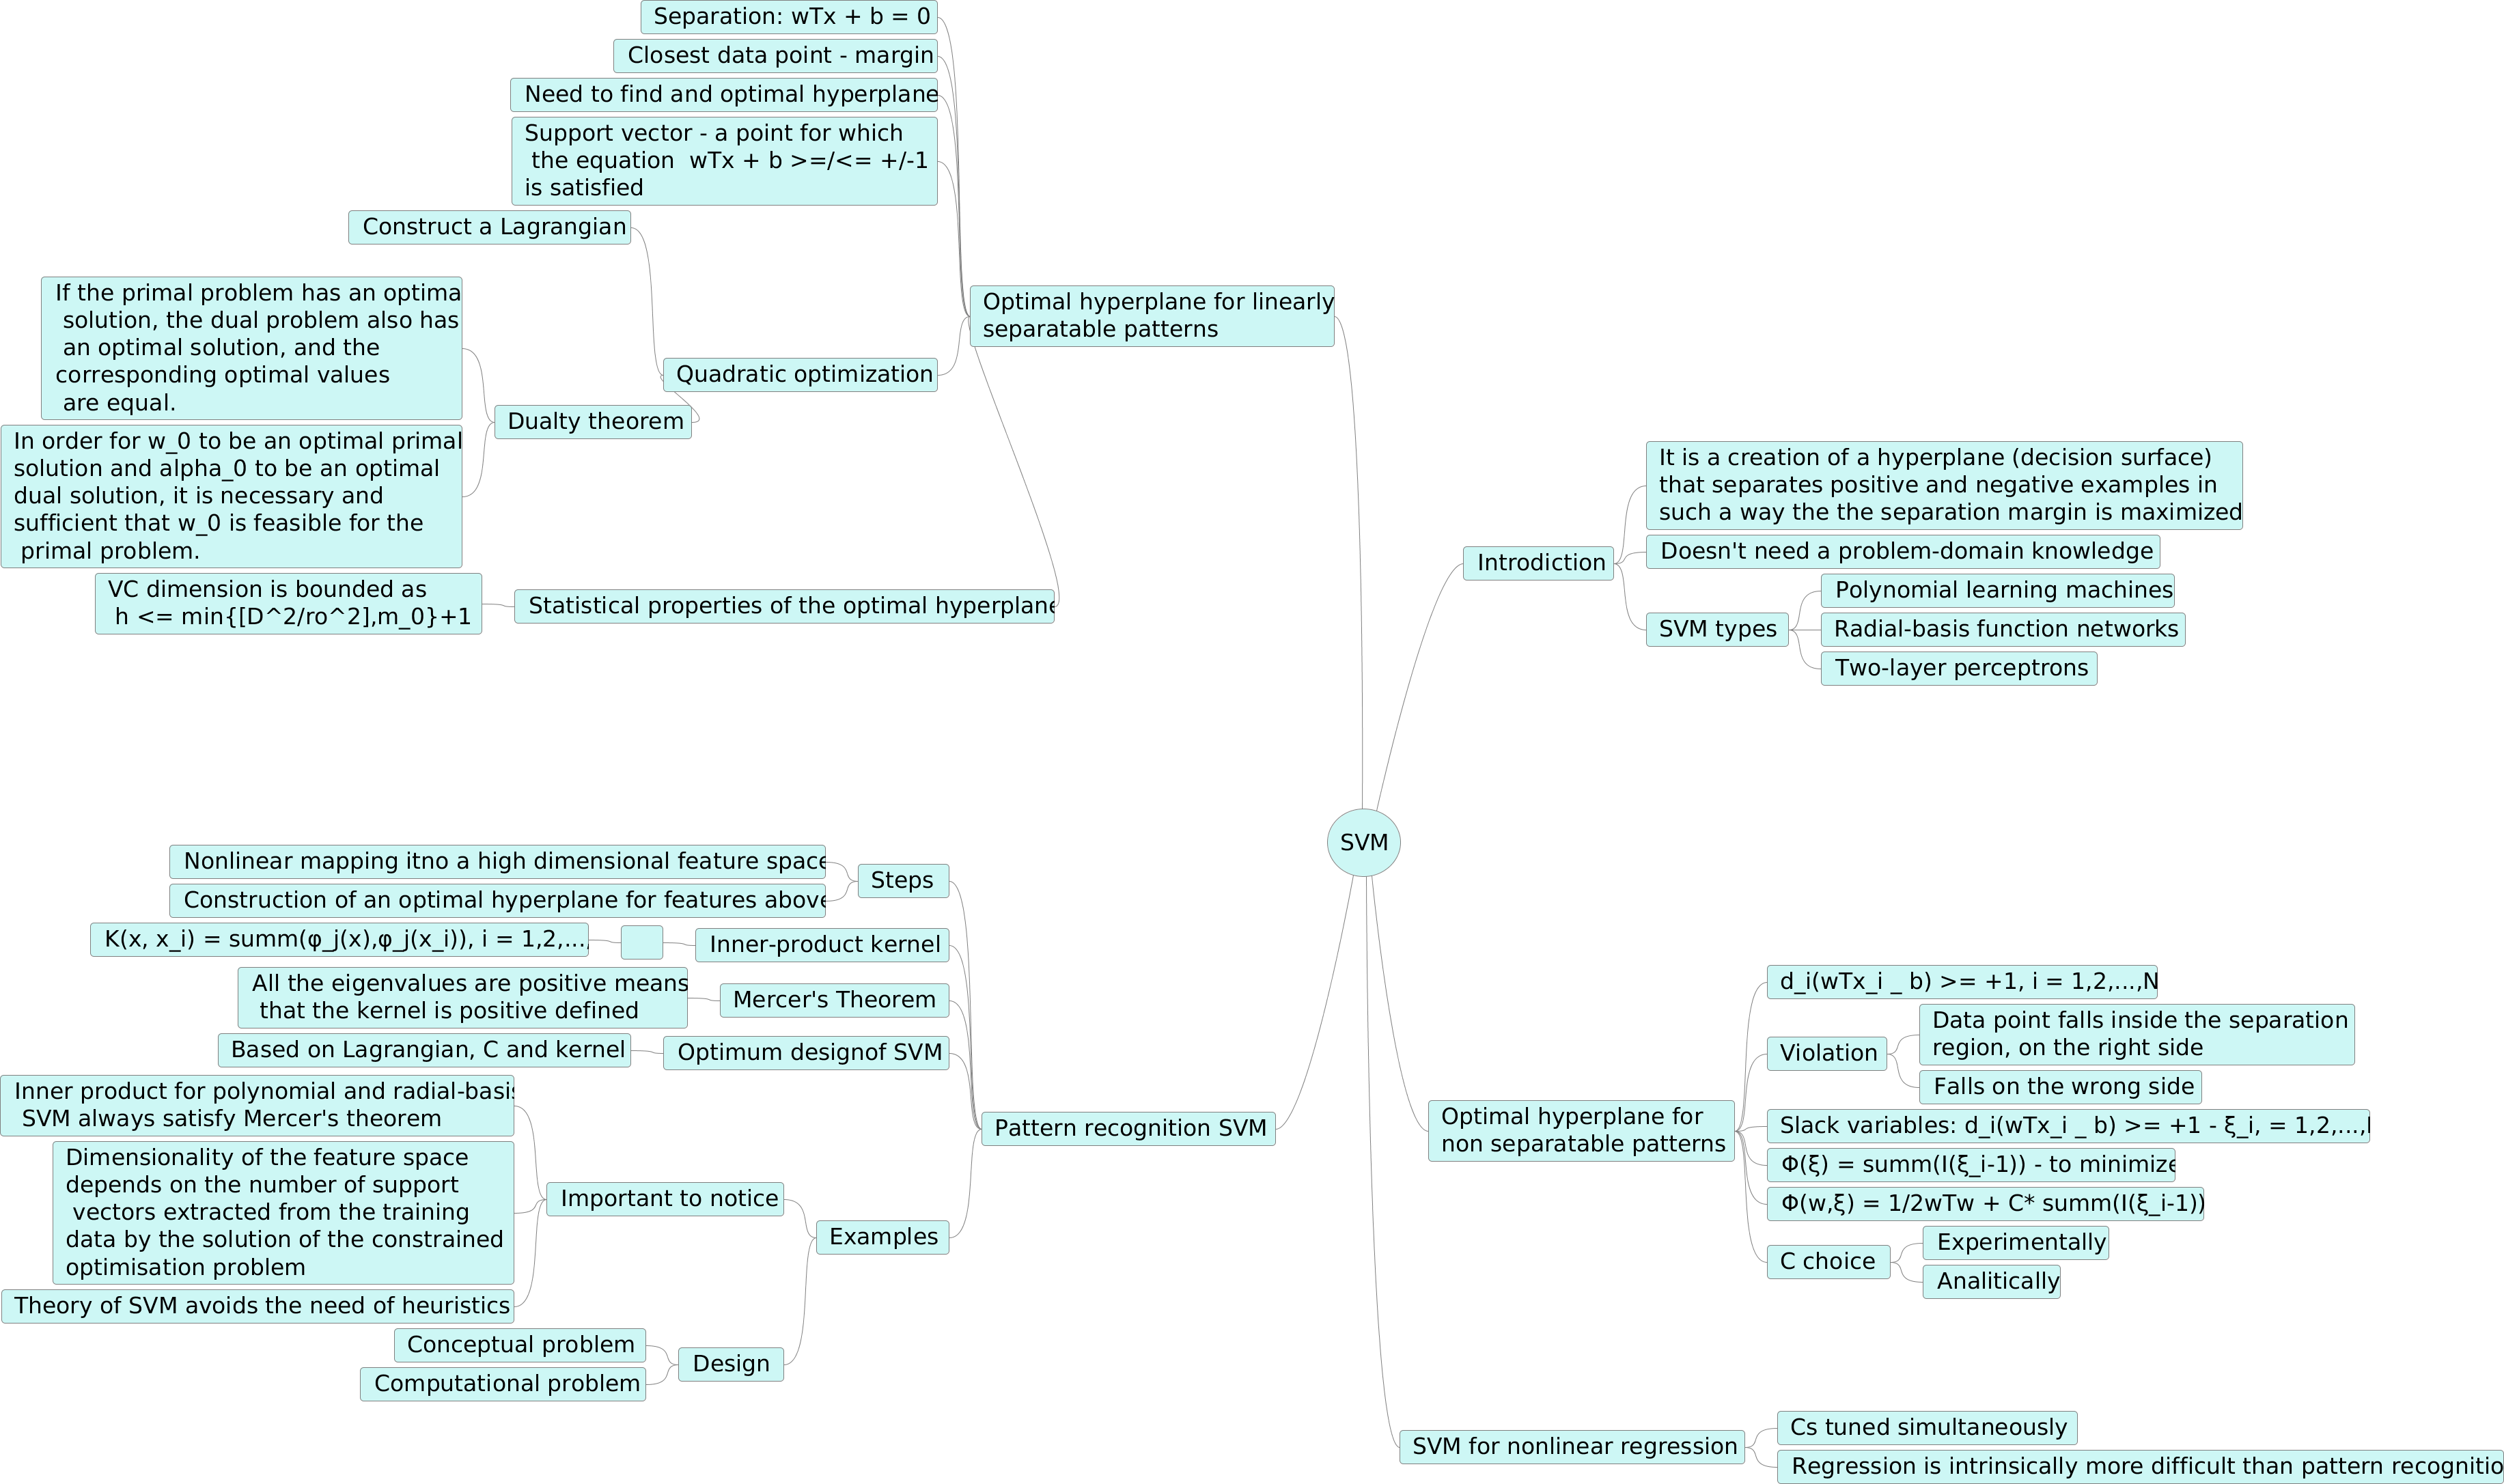
\includegraphics[width=1.0\textwidth]{SVM}
\end{figure}

\section{Exercises}

\subsection{Exercise 2}

The graphs below represent three different one-dimensional classification
(dichotomization) tasks (along a sketched x-axis, dash means "no data point"”). What is the lowest-order polynomial decision function that can correctly classify the given data? Black dots d note class 1 with target function value y1 = +1 and white dots depict class 2 with targets y2 = -1. What are the decision boundaries?\\

\begin{figure}[h!]
  \centering
  \caption{The dots \label{fig:dots}}
  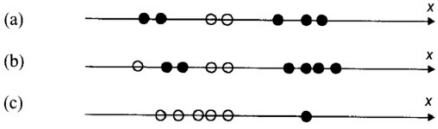
\includegraphics[width=0.5\textwidth]{dots}
\end{figure}

If you wanted to classify the data sets (a), (b), (c) from Fig.\ref{fig:dots} using SVM’s with Gaussian basis functions, how many hidden layer neurons would you need for each problem?\\

Solution:\\

From the positive and negative examples distribution we can assume that (a) requires a second order polynomial function, (b) - third degree and (c) - just a linear one (Fig. \ref{fig:dotsPol}).\\

\begin{figure}[h!]
  \centering
  \caption{The dots with classification polynoms \label{fig:dotsPol}}
  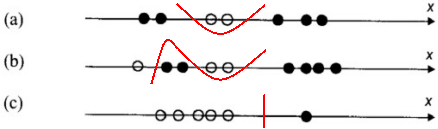
\includegraphics[width=0.5\textwidth]{dotsPol}
\end{figure}

To proof it we used the following code:\\

\lstset{language=Python}
\begin{lstlisting}[frame=single]
from itertools import product

import numpy as np
import matplotlib.pyplot as plt
%matplotlib inline
from sklearn.svm import SVC
import sklearn.svm as svm

Xa = np.array([[1,0],[2,0],[5,0],[6,0],[9,0],[11,0],[12,0]])
ya = np.array([-1, -1, 1, 1, -1, -1,-1])
Xb = np.array([[1,0],[3,0],[4,0],[6,0],[7,0],[10,0],[11,0],[12,0],[14,0]])
yb = np.array([1, -1, -1, 1, 1, -1, -1, -1, -1])
Xc = np.array([[1,0],[2,0],[3,0],[4,0],[5,0],[9,0]])
yc = np.array([1,1,1,1,1,-1])

def classify_and_plot(X,Y, degr):
    clf = svm.SVC(kernel='poly', coef0 = 1, probability=True, degree = degr, gamma=2)
    clf.fit(X, Y)
    x_min, x_max = X[:, 0].min() - 1, X[:, 0].max() + 1
    y_min, y_max = X[:, 1].min() - 1, X[:, 1].max() + 1
    h = 0.1
    x, y = np.meshgrid(np.arange(x_min, x_max, h), np.arange(y_min, y_max, h))
    #print np.c_[xx.ravel(), yy.ravel()]
    Z = clf.predict(np.c_[x.ravel(), y.ravel()])
    Z = Z.reshape(x.shape)
    plt.pcolormesh(x, y, Z, cmap=plt.cm.Paired)
    plt.scatter(X[:, 0], X[:, 1], c=Y, cmap=plt.cm.Paired)
    plt.title('SVM classification')
    plt.axis('tight')
    plt.grid()
    plt.show()
\end{lstlisting}

First, we will try to classify all the cases with degree = 1:

\lstset{language=Python}
\begin{lstlisting}[frame=single]
classify_and_plot(Xa, ya, 1)
classify_and_plot(Xb, yb, 1)
classify_and_plot(Xc, yc, 1)
\end{lstlisting}

The results are shown in Fig. \ref{fig:a1}. We can see that the classification for (c) case is correct, so a linear function is fine for this case. Classifications for (a) and (b) are wrong.\\


\begin{figure}[!htb]
\minipage{0.32\textwidth}
  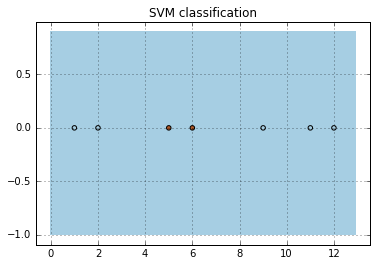
\includegraphics[width=\linewidth]{a1}
  \caption{Classification for (a) case with degree = 1}\label{fig:a1}
\endminipage\hfill
\minipage{0.32\textwidth}
  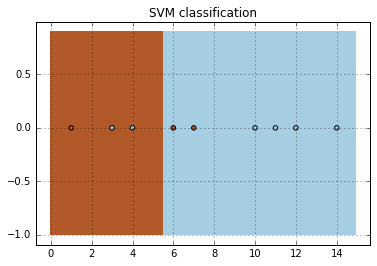
\includegraphics[width=\linewidth]{b1}
  \caption{lassification for (b) case with degree = 1}\label{fig:b1}
\endminipage\hfill
\minipage{0.32\textwidth}%
  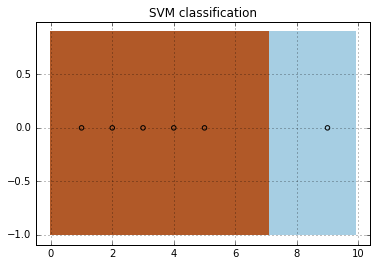
\includegraphics[width=\linewidth]{c1}
  \caption{Alassification for (c) case with degree = 1}\label{fig:c1}
\endminipage
\end{figure}

So, we will test (a) and (b) with degree = 2:
\lstset{language=Python}
\begin{lstlisting}[frame=single]
classify_and_plot(Xa, ya, 2)
classify_and_plot(Xb, yb, 2)
\end{lstlisting}

\begin{figure}[!htb]
\minipage{0.32\textwidth}
  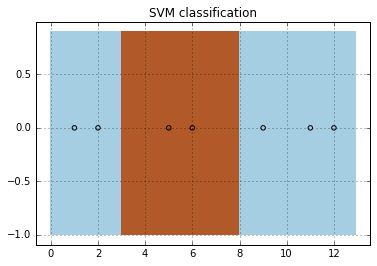
\includegraphics[width=\linewidth]{a2}
  \caption{Classification for (a) case with degree = 2}\label{fig:a2}
\endminipage\hfill
\minipage{0.32\textwidth}
  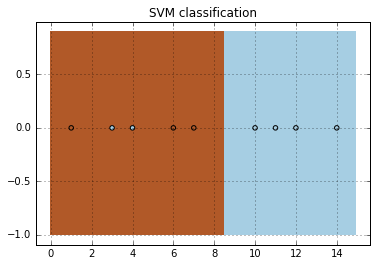
\includegraphics[width=\linewidth]{b2}
  \caption{lassification for (b) case with degree = 2}\label{fig:b2}
\endminipage\hfill
\end{figure}


In Fig. \ref{fig:a2} we see that, as expected, classification for (a) is good, but classification for (b) still failing. So, we need to try degree = 3:
\lstset{language=Python}
\begin{lstlisting}[frame=single]
classify_and_plot(Xb, yb, 3)
\end{lstlisting}

\begin{figure}[!htb]
  \centering
  \caption{Classification for (b) case with degree = 3 \label{fig:b3}}
  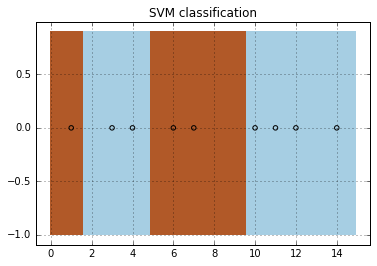
\includegraphics[width=0.3\textwidth]{b3}
\end{figure}


If we wanted to classify the data sets (a), (b), (c) using SVM’s with Gaussian basis functions, we to use another - 'rbf' - kernel function:

\lstset{language=Python}
\begin{lstlisting}[frame=single]
clf = svm.SVC(kernel='rbf', coef0 = 1, probability=True, degree = degr, gamma=2)
\end{lstlisting}

We will obtain the following results:

\begin{figure}[!htb]
\minipage{0.32\textwidth}
  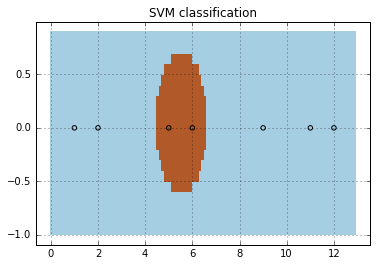
\includegraphics[width=\linewidth]{arbf}
  \caption{Classification for (a) case with Gaussian basis function}\label{fig:arbf}
\endminipage\hfill
\minipage{0.32\textwidth}
  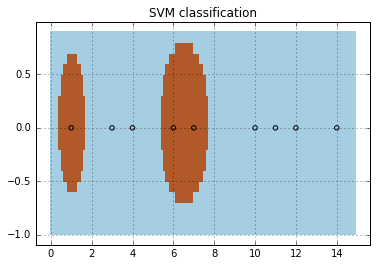
\includegraphics[width=\linewidth]{brbf}
  \caption{lassification for (b) case with Gaussian basis function}\label{fig:brbf}
\endminipage\hfill
\minipage{0.32\textwidth}%
  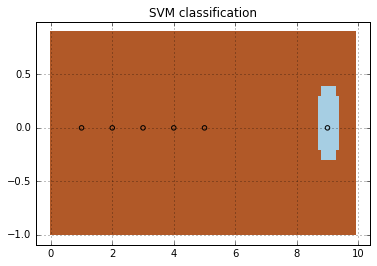
\includegraphics[width=\linewidth]{crbf}
  \caption{Alassification for (c) case with Gaussian basis function}\label{fig:crbf}
\endminipage
\end{figure}

To determine the number of neurons we need a number of features in a feature space that depends on the number of support vectors extracted from the training data. From Fig. \ref{fig:arbf} we can see that in (a) case we have 4 support vectors, in (b) - 6 and in (c) - 2. So, we should have 4, 5 and 2 neurons.

\subsection{Exercise 3}

Download LIVSVM from http://www.csie.ntu.edu.tw/~cjlin/libsvm/. Study how to use it with MATLAB or python. In this exercise you have to use this.
Figure 1.8 on next page shows a pair of �moons� facing each other in an asymmetrically arranged manner. The moon labeled �Region A� is positioned symmetrically with respect to the y-axis, whereas the moon labeled �Region B� is displaced to the right of the y-axis by an amount equal to the radius $r$ and below the x-axis by the distance $d$. The two moons have identical parameters:
\begin{itemize}
\item Radius of each moon, r = 10,
\item Width of each moon, w = 6.
\end{itemize}
The vertical distance d separating the two moons is adjustable; it is measured with respect to the x-axis, as indicated in the figure \ref{fig:moons}.
\begin{itemize}
\item Increasingly positive values of d signify increased separation between the two moons;
\item Increasingly negative values of d signify the two moons� coming closer to each other.
\end{itemize}

\begin{figure}[!htb]

  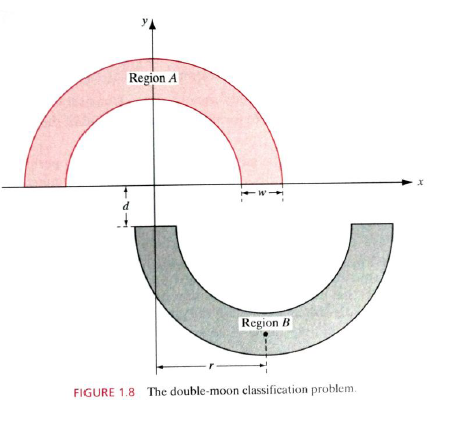
\includegraphics[width=\linewidth]{moons}
  \caption{Data distribution}\label{fig:moons}

\end{figure}
The training sample consists of 1000 pairs of data points, with each pair consisting of one point picked from region A and another point picked from region B, both randomly. The test sample consists of 3,000 pairs of data points, again picked in a random manner.

Tasks:
Your task is to classify the dataset using SVM (Support Vector Machine) for some cases given below. Generate the dataset for each case and classify using different kernels (e.g. linear, polynomial, radial basis etc.) Show the decision boundary (Plotting the classified points using different color will be enough)
\begin{itemize}
\item Case 1: $d = 0$
\item Case 2: $|d| = 1/2 * $(radius of moon�s inner half-circle) and $d$ is negative i.e. d is in the upper side of x-axis.
\item Case 3: Increase $d$ negatively such that both of the moons touch each other.
\item Case 4: Both moons overlap each other
\item Case 5: Add some noise in the training set
\end{itemize}
Try to experiment with different options in svmtrain (LIBSVM). Comment on your findings.
This experiment is taken from Haykin�s book (3rd edition) which is introduced in the first chapter and continued throughout the book (chapter 2, 3, 4). For intuition, you can take a look in it.

Solution to this problem includes 2 MATLAB programs. One is used for double moon data generation. The user can choose number of data points, parameter $d$ and add gaussian noise to data with variance.

\lstinputlisting{generate_moons.m}

The next function uses generated data to train SVM based on chosen kernel type. Then, classification is applied to test data set and finally, uniformly distributed datapoints are classified to find decision boundary.

\lstinputlisting{Ex3.m}

Classification results:

\subsubsection{Case $d = 0$}

The moons can be easily distinguished and hence, separated even with linear kernel with high precision. Other kernels have good results as well.
\begin{figure}[!htb]

  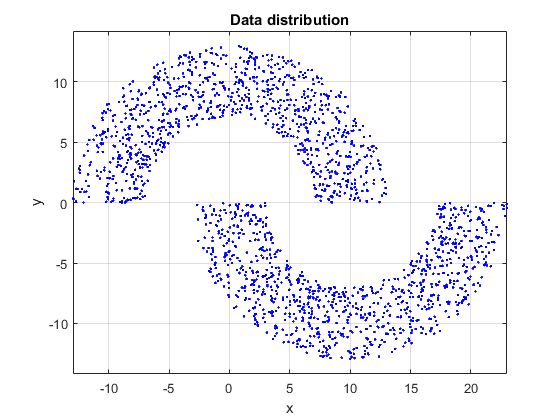
\includegraphics[width=\linewidth]{1poly1}
  \caption{Data distribution}
\end{figure}
\clearpage
\begin{figure}[!htb]
  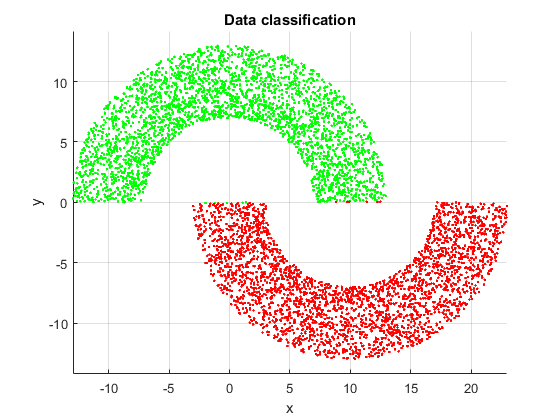
\includegraphics[width=\linewidth]{1lin2}
  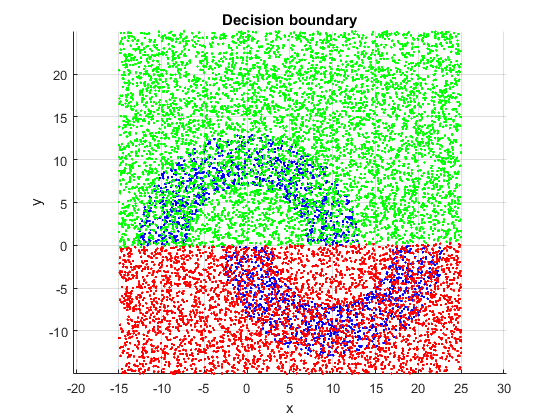
\includegraphics[width=\linewidth]{1lin3}
  \caption{Linear kernel}
\end{figure}
\clearpage
\begin{figure}[!htb]
  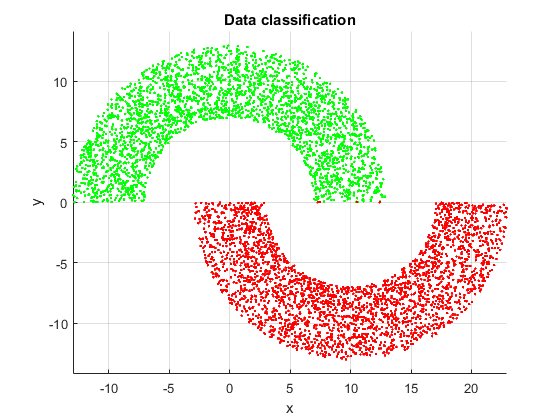
\includegraphics[width=\linewidth]{1poly2}
  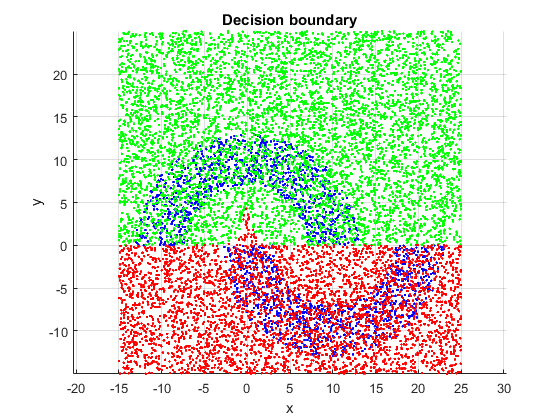
\includegraphics[width=\linewidth]{1poly3}
  \caption{3-rd order polynomial kernel}
\end{figure}
\clearpage
\begin{figure}[!htb]
  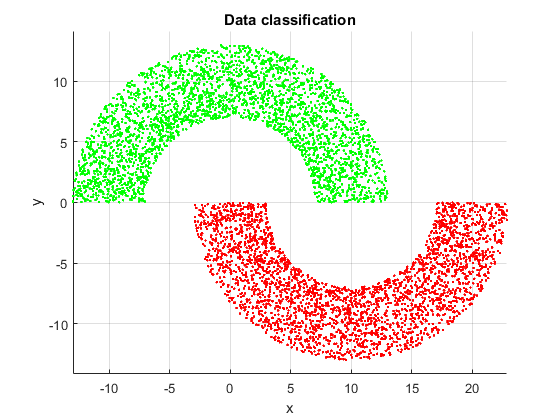
\includegraphics[width=\linewidth]{1rbf2}
  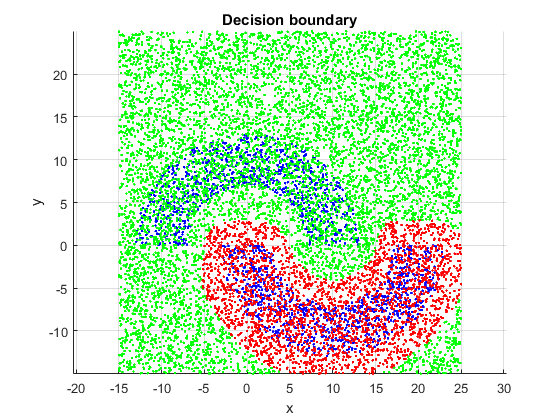
\includegraphics[width=\linewidth]{1rbf3}
  \caption{Gauss kernel}
\end{figure}

\newpage

\subsubsection{Case $d = -3.5$}

In this case moons still can be distinguished, but there is no line that can separate them easily.  So, linear kernel can not cope with it anymore. RBF kernel has the same good performance.



  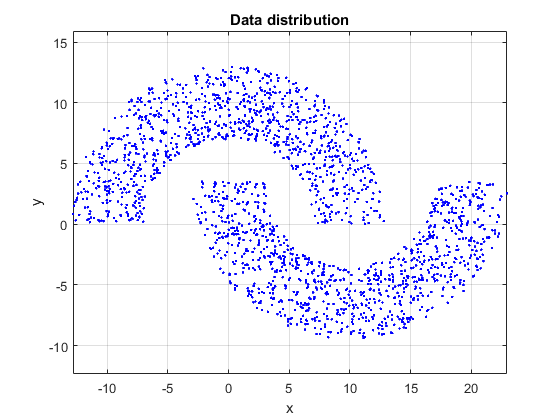
\includegraphics[width=\linewidth]{2lin1}


\clearpage
\begin{figure}[!htb]
  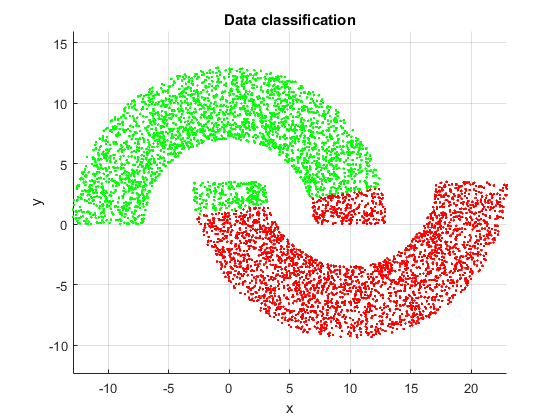
\includegraphics[width=\linewidth]{2lin2}
  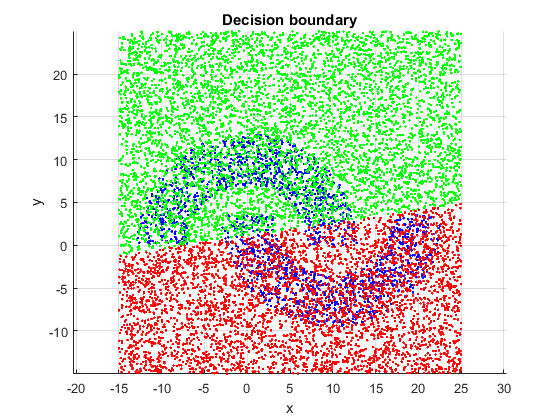
\includegraphics[width=\linewidth]{2lin3}
  \caption{Linear kernel}
\end{figure}
\clearpage
\begin{figure}[!htb]
  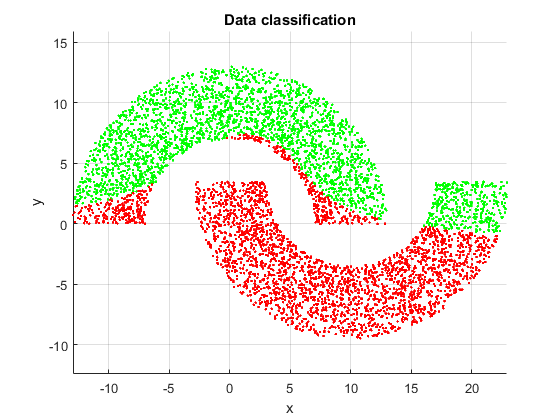
\includegraphics[width=\linewidth]{2poly2}
  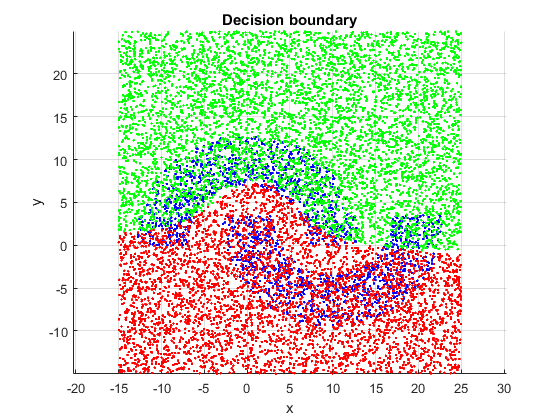
\includegraphics[width=\linewidth]{2poly3}
  \caption{3-rd order polynomial kernel}
\end{figure}
\clearpage
\begin{figure}[!htb]
  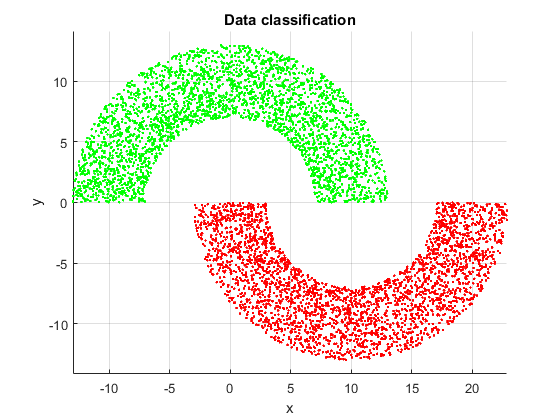
\includegraphics[width=\linewidth]{1rbf2}
  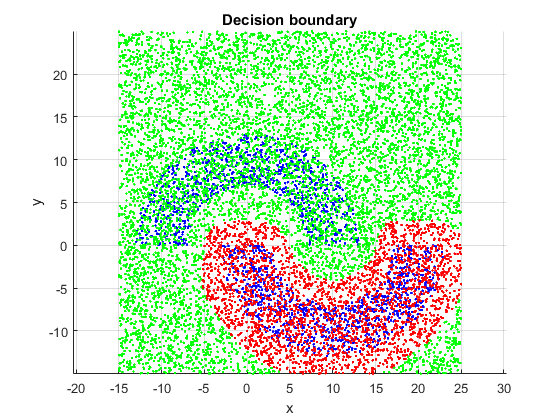
\includegraphics[width=\linewidth]{1rbf3}
  \caption{Gauss kernel kernel}
\end{figure}

\newpage

\subsubsection{Case $d = -7$. Moons slightly connected}

In this case moons are connected but still can be divided. Linear and polynomial kernel work worse that RBF kernel.

  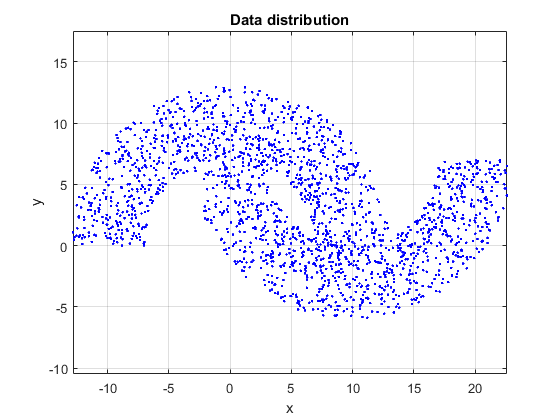
\includegraphics[width=\linewidth]{3lin1}

\clearpage
\begin{figure}[!htb]
  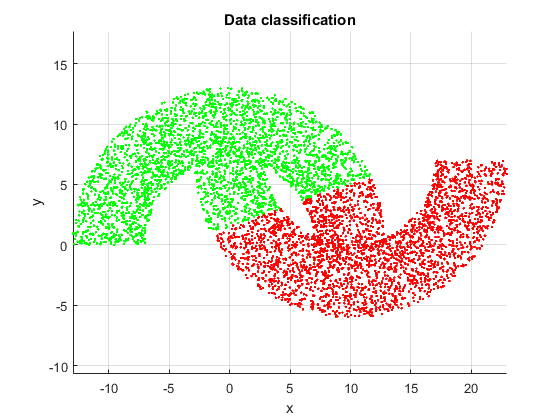
\includegraphics[width=\linewidth]{3lin2}
  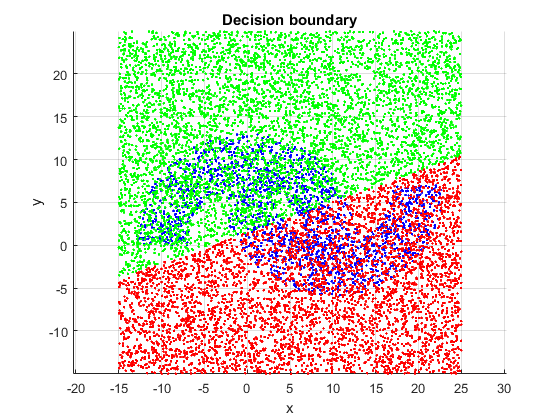
\includegraphics[width=\linewidth]{3lin3}
  \caption{Linear kernel}
\end{figure}
\clearpage
\begin{figure}[!htb]
  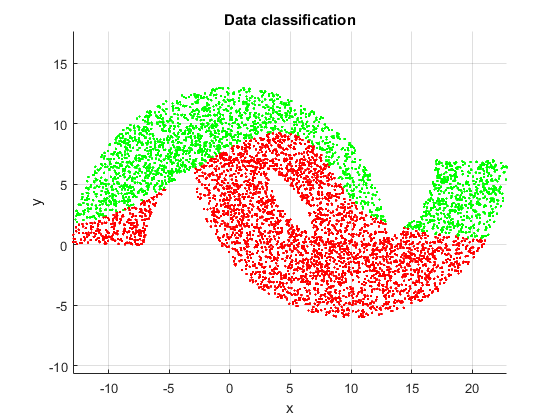
\includegraphics[width=\linewidth]{3poly2}
  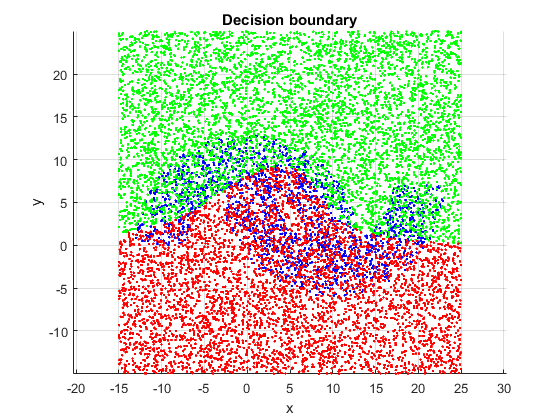
\includegraphics[width=\linewidth]{3poly3}
  \caption{3-rd order polynomial kernel}
\end{figure}
\clearpage
\begin{figure}[!htb]
  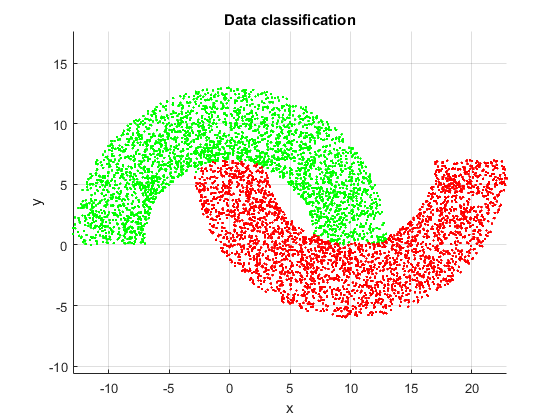
\includegraphics[width=\linewidth]{3rbf2}
  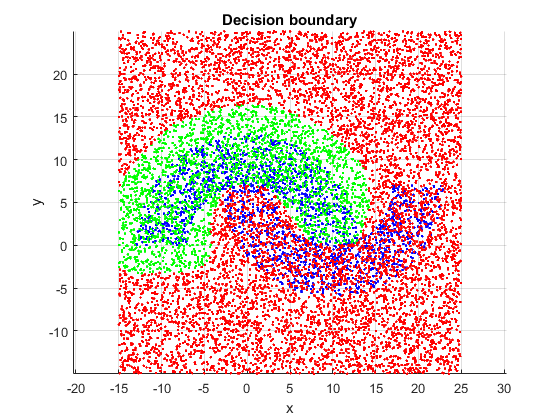
\includegraphics[width=\linewidth]{3rbf3}
  \caption{Gauss kernel }
\end{figure}

\newpage

\subsubsection{Case $d = -13$. Moons overlay}

Moons can not be recognized by eyesight. All kernels, except RBF kernel show bad performance. RBF has accuracy around 78\%. This accuracy do not grow with extra training data.



  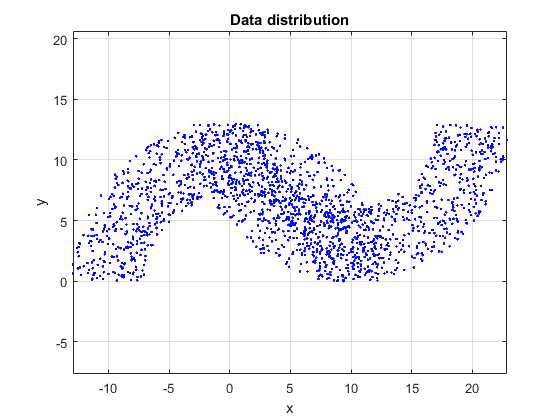
\includegraphics[width=\linewidth]{4poly1}
\clearpage

\begin{figure}[!htb]
  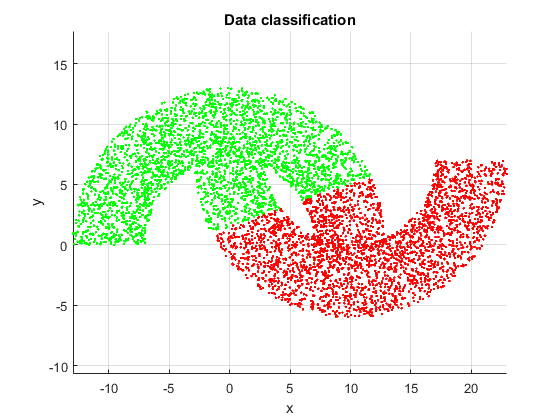
\includegraphics[width=\linewidth]{3lin2}
  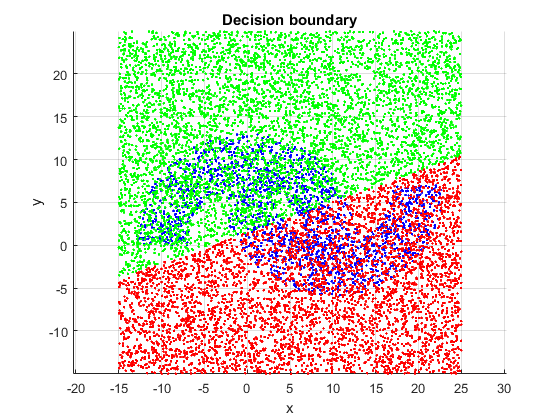
\includegraphics[width=\linewidth]{3lin3}
  \caption{Linear kernel}
\end{figure}
\clearpage
\newpage

Gauss kernel.
  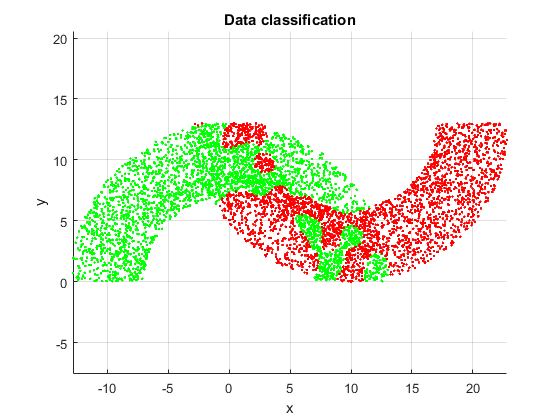
\includegraphics[width=\linewidth]{4rbf2}
  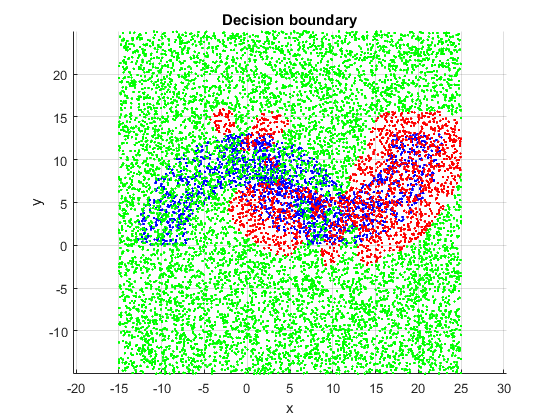
\includegraphics[width=\linewidth]{4rbf3}



\newpage
\subsubsection{Case noise}

Noise can spoil even the easiest example. With $d=0$, linear kernel already has troubles

  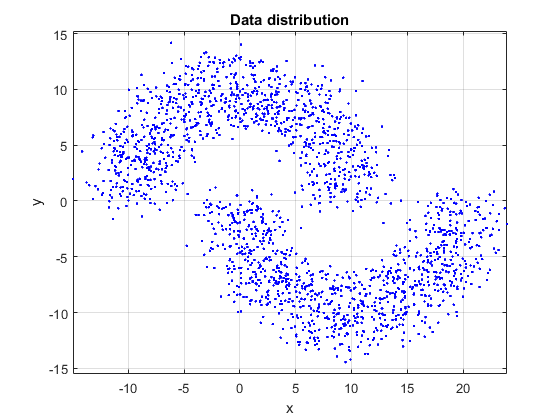
\includegraphics[width=\linewidth]{1lin1n}

\clearpage

  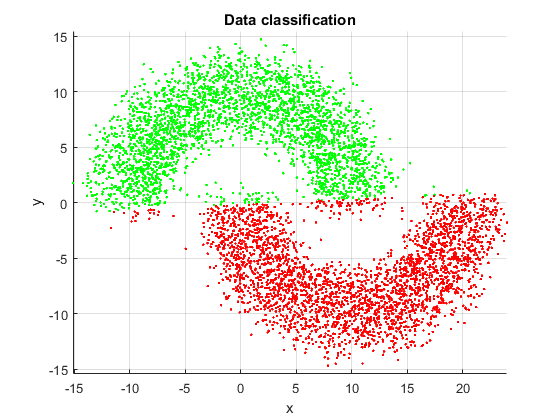
\includegraphics[width=\linewidth]{1lin2n}
  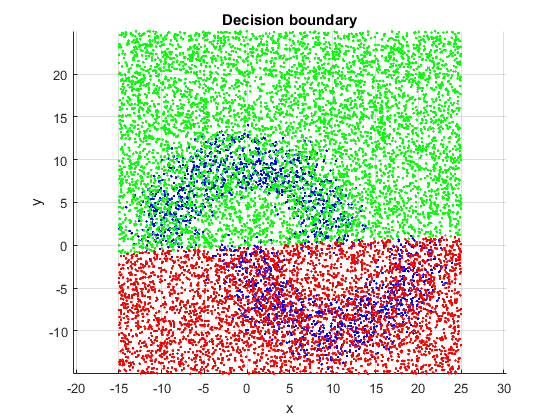
\includegraphics[width=\linewidth]{1lin3n}

\newpage
\subsubsection{The hardest case}
Overlapping moons and noise. RBF kernel SVM still shown good results.


\begin{figure}[!hb]
  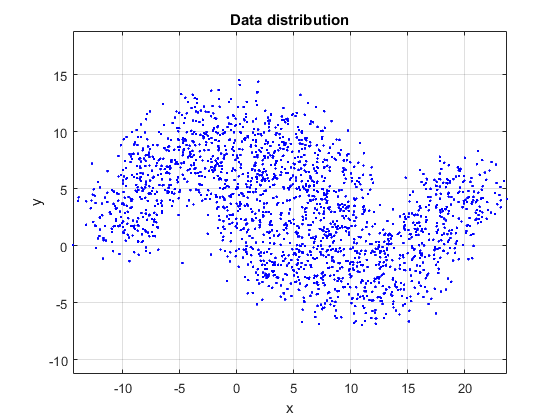
\includegraphics[width=\linewidth]{5rbf1}
  \caption{Data distribution}
\end{figure}
\clearpage


\begin{figure}[!hb]
  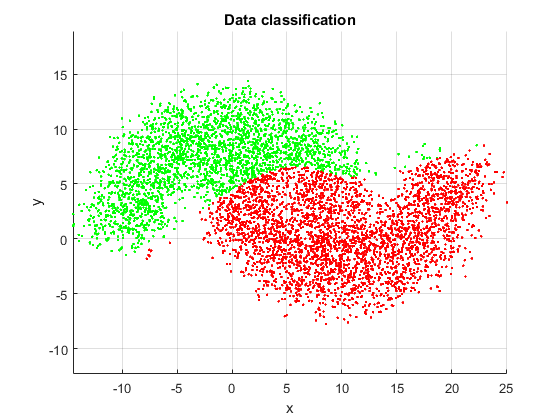
\includegraphics[width=\linewidth]{5poly2}
  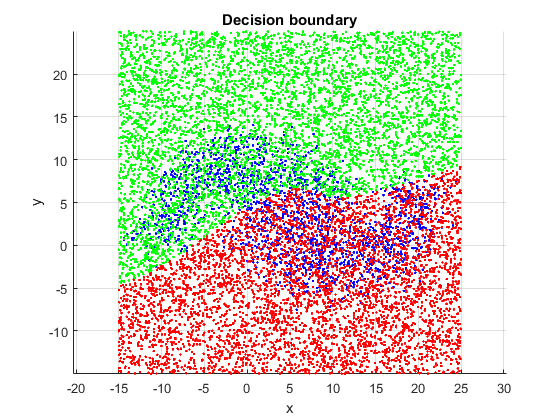
\includegraphics[width=\linewidth]{5poly3}
  \caption{3-rd order polynomial kernel}
\end{figure}
\clearpage
\begin{figure}[!hb]
  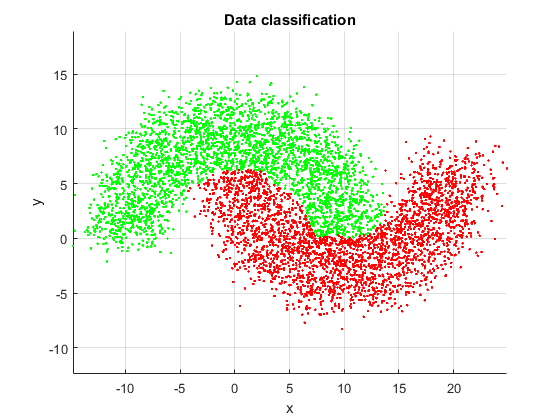
\includegraphics[width=\linewidth]{5rbf2}
  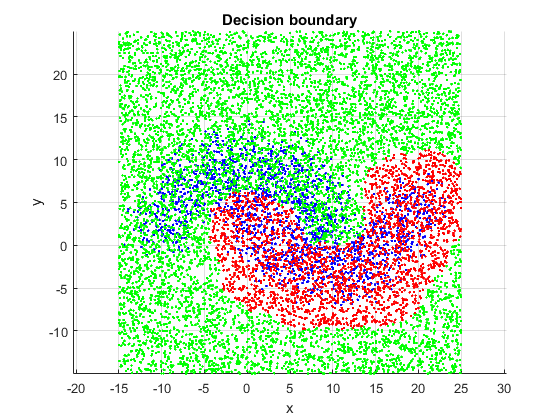
\includegraphics[width=\linewidth]{5rbf3}
  \caption{Gauss kernel }
\end{figure}
\clearpage


\newpage
\subsubsection{Results}
\begin{itemize}
\item In case with two moons RBF kernel has the best classification abilities. 
\item It also shown good computational efficiency.
\item Linear classification is really cheap but useless.
\item Polynomial kernel are really expensive and usually worse that RBF.
\end{itemize}

\end{document}
